% Soubory musí být v kódování, které je nastaveno v příkazu \usepackage[...]{inputenc}

\documentclass[%        Základní nastavení
  %draft,    				  % Testovací překlad
  12pt,       				% Velikost základního písma je 12 bodů
	t,                  % obsah slajdů bude vždy začínat od shora (nebude vertikálně centrovaný)
	aspectratio=1610,   % poměr stran bude 16:10
	unicode,						% Záložky a informace budou v kódování unicode
]{beamer}				    	% Dokument třídy beamer

\usepackage[utf8]		  % Kódování zdrojových souborů je v UTF-8
	{inputenc}

\usepackage{graphicx}
\usepackage[nohyperlinks]{acronym}
\usepackage{booktabs}
\usepackage{amsmath}
\usepackage{tikz}
\usetikzlibrary{positioning, arrows.meta, calc}
\usepackage{cmap}

%%%%%%%%%%%%%%%%%%%%%%%%%%%%%%%%%%%%%%%%%%%%%%%%%%%%%%%%%%%%%%%%%
%%%%%%      Definice informací o dokumentu             %%%%%%%%%%
%%%%%%%%%%%%%%%%%%%%%%%%%%%%%%%%%%%%%%%%%%%%%%%%%%%%%%%%%%%%%%%%%

% V tomto souboru se nastavují téměř veškeré informace, proměnné mezi studenty:
% jméno, název práce, pohlaví atd.
% Tento soubor je SDÍLENÝ mezi textem práce a prezentací k obhajobě -- netřeba něco nastavovat na dvou místech.

\usepackage[
%%% Z následujících voleb jazyka lze použít pouze jednu
  czech-english,		% originální jazyk je čeština, překlad je anglicky (výchozí)
  %english-czech,	% originální jazyk je angličtina, překlad je česky
  %slovak-english,	% originální jazyk je slovenština, překlad je anglicky
  %english-slovak,	% originální jazyk je angličtina, překlad je slovensky
%
%%% Z následujících voleb typu práce lze použít pouze jednu
  %semestral,		  % semestrální práce (výchozí)
  %bachelor,			%	bakalářská práce
  master,			  % diplomová práce
  %treatise,			% pojednání o disertační práci
  %doctoral,			% disertační práce
%
%%% Z následujících voleb zarovnání objektů lze použít pouze jednu
%  left,				  % rovnice a popisky plovoucích objektů budou zarovnány vlevo
	center,			    % rovnice a popisky plovoucích objektů budou zarovnány na střed (vychozi)
%
%%% Níže uvedený přepinač 'electronic' lze použít pro generování elektronické verze práce; pokud je aktivní, vnější a vnitřní okraj sazebního obrazce budou shodné pro liché i sudé stránky.
% Pozor, neplést si s volbou oneside/twoside!
% Pozor, pro tiskovou verzi nechejte vypnuté!
%	electronic			
]{thesis}   % Balíček pro sazbu studentských prací


%%% Jméno a příjmení autora ve tvaru
%  [tituly před jménem]{Křestní}{Příjmení}[tituly za jménem]
% Pokud osoba nemá titul před/za jménem, smažte celý řetězec '[...]'
\author[Bc.]{Dušan}{Horák}

%%% Identifikační číslo autora (VUT ID)
\butid{230076}

%%% Pohlaví autora/autorky
% (nepoužije se ve variantě english-czech ani english-slovak)
% Číselná hodnota: 1...žena, 0...muž
\gender{0}

%%% Jméno a příjmení vedoucího/školitele včetně titulů
%  [tituly před jménem]{Křestní}{Příjmení}[tituly za jménem]
% Pokud osoba nemá titul před/za jménem, smažte celý řetězec '[...]'
\advisor[Ing.]{Libor}{Veselý}[Ph.D.]

%%% Jméno a příjmení oponenta včetně titulů
%  [tituly před jménem]{Křestní}{Příjmení}[tituly za jménem]
% Pokud osoba nemá titul před/za jménem, smažte celý řetězec '[...]'
% Nastavení oponenta se uplatní pouze v prezentaci k obhajobě;
% v případě, že nechcete, aby se na titulním snímku prezentace zobrazoval oponent, pouze příkaz zakomentujte;
% u obhajoby semestrální práce se oponent nezobrazuje (jelikož neexistuje)
% U dizertační práce jsou typicky dva až tři oponenti. Pokud je chcete mít na titulním slajdu, prosím ručně odkomentujte a upravte jejich jména v definici "VUT title page" v souboru thesis.sty.
\opponent[Ing.]{Lukáš}{Pohl}[Ph.D.]

%%% Název práce
%  Parametr ve složených závorkách {} je název v originálním jazyce,
%  parametr v hranatých závorkách [] je překlad (podle toho jaký je originální jazyk).
%  V případě, že název Vaší práce je dlouhý a nevleze se celý do zápatí prezentace, použijte příkaz
%  \def\insertshorttitle{Zkác.\ náz.\ práce}
%  kde jako parametr vyplníte zkrácený název. Pokud nechcete zkracovat název, budete muset předefinovat,
%  jak se vytváří patička slidu. Viz odkaz: https://bit.ly/3EJTp5A
\title[Field-oriented control of five-phase permanent magnet synchronous motor]{Vektorové řízení pětifázového synchronního motoru s permanentními magnety}

%%% Označení oboru studia
%  Parametr ve složených závorkách {} je název oboru v originálním jazyce,
%  parametr v hranatých závorkách [] je překlad
\specialization[Teleinformatics]{Teleinformatika}

%%% Označení ústavu
%  Parametr ve složených závorkách {} je název ústavu v originálním jazyce,
%  parametr v hranatých závorkách [] je překlad
\department[Department of Control and Instrumentation]{Ústav automatizace a měřicí techniky}
%\department[Department of Biomedical Engineering]{Ústav biomedicínského inženýrství}
%\department[Department of Electrical Power Engineering]{Ústav elektroenergetiky}
%\department[Department of Electrical and Electronic Technology]{Ústav elektrotechnologie}
%\department[Department of Physics]{Ústav fyziky}
%\department[Department of Foreign Languages]{Ústav jazyků}
%\department[Department of Mathematics]{Ústav matematiky}
%\department[Department of Microelectronics]{Ústav mikroelektroniky}
%\department[Department of Radio Electronics]{Ústav radioelektroniky}
%\department[Department of Theoretical and Experimental Electrical Engineering]{Ústav teoretické a experimentální elektrotechniky}
%\department[Department of Telecommunications]{Ústav telekomunikací}
%\department[Department of Power Electrical and Electronic Engineering]{Ústav výkonové elektrotechniky a elektroniky}

%%% Označení fakulty
%  Parametr ve složených závorkách {} je název fakulty v originálním jazyce,
%  parametr v hranatých závorkách [] je překlad
%\faculty[Faculty of Architecture]{Fakulta architektury}
\faculty[Faculty of Electrical Engineering and~Communication]{Fakulta elektrotechniky a~komunikačních technologií}
%\faculty[Faculty of Chemistry]{Fakulta chemická}
%\faculty[Faculty of Information Technology]{Fakulta informačních technologií}
%\faculty[Faculty of Business and Management]{Fakulta podnikatelská}
%\faculty[Faculty of Civil Engineering]{Fakulta stavební}
%\faculty[Faculty of Mechanical Engineering]{Fakulta strojního inženýrství}
%\faculty[Faculty of Fine Arts]{Fakulta výtvarných umění}
%
%Nastavení logotypu (v hranatych zavorkach zkracene logo, ve slozenych plne):
\facultylogo[logo/FEKT_zkratka_barevne_PANTONE_CZ]{logo/png2pdf}

%%% Rok odevzdání práce
\graduateyear{2026}
%%% Akademický rok odevzdání práce
\academicyear{2025/26}

%%% Datum obhajoby (uplatní se pouze v prezentaci k obhajobě)
\date{10.\,06.\,2026} 

%%% Místo obhajoby
% Na titulních stránkách bude automaticky vysázeno VELKÝMI písmeny (pokud tyto stránky sází šablona)
\city{Brno}

%%% Abstrakt
\abstract[%
This thesis presents the design and implementation of field-oriented control of a five-phase interior permanent magnet synchronous motor (IPMSM).

Five-phase motors achieve higher torque density, smoother torque ripple, and greater fault tolerance compared to their three-phase equivalents. To describe these motors, an extended Clarke and Park transformation into the $dq_{1\,3}$ space is introduced, decomposing motor quantities into two parallel planes --- $dq_1$ capturing the fundamental harmonic component and $dq_3$ capturing its third harmonic. A motor model suitable for controller design is derived using this transformation.

The motor is driven by space vector pulse width modulation (SVPWM) with a symmetric vector arrangement. A cascade control structure is designed, consisting of an inner current loop and an outer speed loop. Back-EMF compensation is verified in the current loop, reducing overshoots during step changes of the reference value.

Reference currents are generated by the Maximum Torque Per Ampere (MTPA) algorithm, maximising the torque produced per ampere drawn from the supply. Third harmonic injection is also implemented, increasing the theoretical maximum torque by approximately 20\,\% compared to control utilising only the fundamental harmonic subspace. Current references are precomputed into a lookup table to reduce the online computational burden.

The designed algorithms are implemented and verified in Matlab/Simulink, both on a custom analytical model and on a Simscape model. The control blocks are subsequently adapted for HDL code generation using the Matlab HDL Coder and HDL Verifier toolboxes. The generated IP cores are deployed and functionally verified on the ZedBoard development kit (SoC Xilinx Zynq-7000). The implemented solution utilises approximately 90\,\% of the available FPGA logic resources.
]{%
Diplomová práce se zabývá návrhem a implementací vektorového řízení pětifázového
synchronního motoru s permanentními magnety umístěnými uvnitř rotoru (IPMSM).

Pětifázové motory oproti třífázovým dosahují vyšší hustoty točivého momentu,
plynulejšího průběhu a větší odolnosti vůči poruchám. Pro jejich popis je
představena rozšířená Clarkova a Parkova transformace do prostoru $dq_{1\,3}$,
která motorové veličiny rozděluje do dvou rovnoběžných rovin -- $dq_1$ zachycující
1. harmonickou složku a $dq_3$ zachycující její trojnásobek. Pomocí této
transformace je odvozen model motoru vhodný pro návrh regulátorů.

Pro buzení motoru je použita prostorově vektorová pulzně šířková modulace (SVPWM)
se symetrickým uspořádáním vektorů. Je navrženo kaskádní řízení složené
z vnitřní proudové smyčky a vnější smyčky otáčkové. V proudové smyčce je ověřena
kompenzace zpětně indukovaného elektromotorického napětí, která snižuje překmity
při skokové změně žádané hodnoty.

Referenční proudy jsou generovány algoritmem MTPA (Maximum Torque Per Ampere),
zajišťujícím maximální moment na odebíraný ampér ze zdroje. Dále je implementována
injekce 3. harmonické, která teoretický maximální moment zvyšuje přibližně
o 20\,\% oproti řízení využívajícímu pouze prostor 1. harmonické. Proudové
reference jsou předpočítány do vyhledávací tabulky, čímž se snižuje výpočetní
náročnost za běhu.

Navržené algoritmy jsou implementovány a ověřeny v prostředí Matlab/Simulink,
a to jak na vlastním analytickém modelu, tak na modelu ze knihovny Simscape.
Řídicí bloky jsou následně přizpůsobeny pro generování HDL kódu pomocí Matlab
HDL Coder a HDL Verifier toolboxů. Vygenerovaná IP jádra jsou nahrána
a funkčně ověřena na vývojovém kitu ZedBoard (SoC Xilinx Zynq-7000).
Navržené řešení využívá přibližně 90\,\% dostupných logických zdrojů FPGA.

  }

%%% Klíčová slova
\keywrds[ 
  field oriented controll, spacevector pulse width modulation, 5pahse permanent magnet synchronous motor
]{%
vektorové řízení, 5-tifázová motor s permantními magnety, prostorově voektorová pulzně šířková modulce
}

%%% Poděkování
\acknowledgement{%
Rád bych poděkoval vedoucímu diplomové práce
panu Ing.~Liboru Veslému, Ph.D.\ za odborné vedení,
konzultace, trpělivost a~podnětné návrhy k~práci.
}%

%%%%%%%%%%%%%%%%%%%%%%%%%%%%%%%%%%%%%%%%%%%%%%%%%%%%%%%%%%%%%%%%%%%%%%%%
%%%%%%     Nastavení polí ve Vlastnostech dokumentu PDF      %%%%%%%%%%%
%%%%%%%%%%%%%%%%%%%%%%%%%%%%%%%%%%%%%%%%%%%%%%%%%%%%%%%%%%%%%%%%%%%%%%%%
\pdfsettings
\hypersetup{pdfpagemode=FullScreen}
%%%%%%%%%%%%%%%%%%%%%%%%%%%%%%%%%%%%%%%%%%%%%%%%%%%%%%%%%%%%%%%%%%%%%%%

\usetheme{VUT}
\logoheader

\begin{document}

\disablenavigationsymbols

% Titulní snímek
\maketitle

%%%%%%%%%%%%%%%%%%%%%%%%%%%%%%%%%%%%%%%%%%%%%%%%%%%%%%%%%%%%%%%%%%%%%%%
% Snímek 1: Cíle práce
\begin{frame}
	\frametitle{Cíle práce}
	\begin{itemize}
		\item Nastudovat problematiku \textbf{vektorového řízení pětifázového PMSM}
		\item Odvodit a implementovat transformaci do prostoru $dq_{1\,3}$
		\item Popsat/navrhout  \textbf{SVPWM modulátor}  
		\item Implementovat algoritmus \textbf{vektorového řízení} v prostředí Matlab/ Simulink
		\item Implementovat na  vývojovém kitu \textbf{ZedBoard (Xilinx Zynq-7000)}
	\end{itemize}
\end{frame}

% Snímek 2: Pětifázový motor
\begin{frame}
	\frametitle{Pětifázový synchronní motor s permanentními magnety }
	
	\begin{figure}
		\centering
		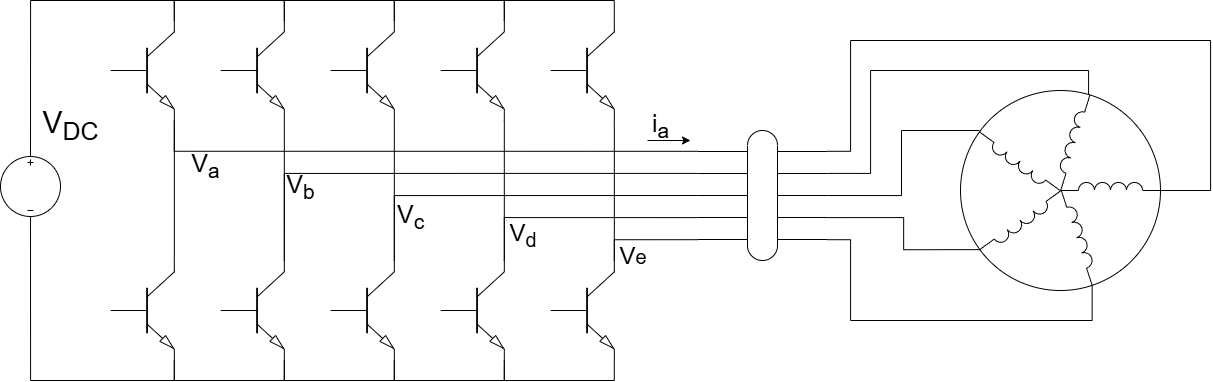
\includegraphics[width=0.85\textwidth]{obrazky/electric.drawio (1).png}
	\end{figure}	
	
	\textbf{Výhody oproti třífázovému motoru:}
	\begin{itemize}
		\item Vyšší hustota točivého momentu
		\item Plynulejší průběh momentu
		\item Schopné provozu, odolnost při poruše
	\end{itemize}	
	
	
	
	
\end{frame}			




% Matematický popis motoru
\begin{frame}
	\begin{columns}[T]
		\begin{column}{0.4\textwidth}
			\frametitle{Matematický popis motoru}
			\textbf{Statorové napětí:}
			\begin{equation*}
				v=R_s i + \frac{d\psi_s}{dt} 
			\end{equation*}

	
	
	\begin{equation*}
		\label{eq:flux rotace abc} 
		\psi_m(\theta)  = 
		\underbrace{
			\begin{bmatrix}
				\cos \theta_r \\
				\cos(\theta_r - 2\pi/5) \\
				\cos(\theta_r - 4\pi/5) \\
				\cos(\theta_r + 4\pi/5) \\
				\cos(\theta_r + 2\pi/5)
			\end{bmatrix}}_\gamma
			\cdot \Psi_{PM}
		\end{equation*}
	\end{column}

	\begin{column}{0.5\textwidth}
		\textbf{Statorový tok:}
			\begin{equation*}
			\psi_s = L_s(\theta) i + \psi_m(\theta)
			\end{equation*}
		\begin{equation*}
			\label{eq:model abc induknost}
			L_{s}(\theta) = L_{ls}I + L_{A5}M_{a5} + L_{B}M_{b5}(\theta)
		\end{equation*}
			{

\begin{equation*}
    \resizebox{0.9\textwidth}{!}{$
        M_{b5}=
        \begin{bmatrix}
         \cos\left(2\,\theta \right) & \cos\left(\frac{2\,\pi}{5}-2\,\theta \right) & \cos\left(\frac{4\,\pi}{5}-2\,\theta \right) & \cos\left(\frac{4\,\pi}{5}+2\,\theta \right) & \cos\left(\frac{2\,\pi}{5}+2\,\theta \right)\\ \cos\left(\frac{2\,\pi}{5}-2\,\theta \right) & \cos\left(\frac{4\,\pi}{5}-2\,\theta \right) & \cos\left(\frac{4\,\pi}{5}+2\,\theta \right) & \cos\left(\frac{2\,\pi}{5}+2\,\theta \right) & \cos\left(2\,\theta \right)\\ \cos\left(\frac{4\,\pi}{5}-2\,\theta \right) & \cos\left(\frac{4\,\pi}{5}+2\,\theta \right) & \cos\left(\frac{2\,\pi}{5}+2\,\theta \right) & \cos\left(2\,\theta \right) & \cos\left(\frac{2\,\pi}{5}-2\,\theta \right)\\ \cos\left(\frac{4\,\pi}{5}+2\,\theta \right) & \cos\left(\frac{2\,\pi}{5}+2\,\theta \right) & \cos\left(2\,\theta \right) & \cos\left(\frac{2\,\pi}{5}-2\,\theta \right) & \cos\left(\frac{4\,\pi}{5}-2\,\theta \right)\\ \cos\left(\frac{2\,\pi}{5}+2\,\theta \right) & \cos\left(2\,\theta \right) & \cos\left(\frac{2\,\pi}{5}-2\,\theta \right) & \cos\left(\frac{4\,\pi}{5}-2\,\theta \right) & \cos\left(\frac{4\,\pi}{5}+2\,\theta \right) 
        \end{bmatrix}
        $}
\end{equation*} 
}
	\end{column}
\end{columns}
\vspace{0.5ex}
{\small  $\psi_s$~-- statorový tok, $\psi_m$~-- tok PM, $L_{ls}$~-- rozptylová indukčnost, $L_{A5}$, $L_B$~-- amplitudy indukčností, $M_{a5}$, $M_{b5}$~-- matice indukčností, $\Psi_{PM}$~-- amplituda toku PM}

\end{frame}


% dq_13
\begin{frame}
	\frametitle{Transformace do prostoru $dq_{1\,3}$}
	\begin{columns}
		\begin{column}{0.4\textwidth}
			\textbf{Převod do $\alpha \beta_{1\,3}$}
			\[	f_{\alpha_1 \beta_1 } \equiv \frac{2}{5} \left( f_{a} + a_5 f_{b} + a_5^2 f_{c} + a_5^3 f_{d} + a_5^4 f_{e} \right)
			\]
			\[	f_{\alpha_3 \beta_3 } \equiv \frac{2}{5} \left( f_{a} + a_5 f_{c} + a_5^2 f_{e} + a_5^3 f_{b} + a_5^4 f_{d} \right)
			\]
			\[  	\begin{gathered}
					f_0=\frac{1}{5}\left( f_a +f_b+f_c+f_d+f_e\right)\\
					a_5=e^{j2\pi/5}
			\end{gathered}
			\]

			\textbf{Převod do $d q_{1\,3}$}
			\[	f_{d_1 q_1}= f_{\alpha_1 \beta_1} \cdot e^{-j\theta}\]
			\[	f_{d_3 q_3}= f_{\alpha_3 \beta_3} \cdot e^{-j3\theta}\]
		\end{column}
		\begin{column}{0.6\textwidth}
			\begin{figure}
				\centering
				

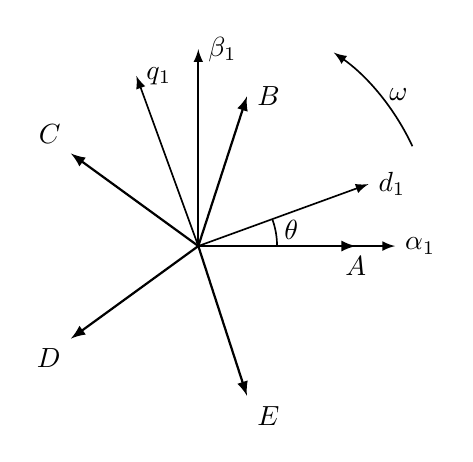
\begin{tikzpicture}[>=latex, line width=0.6pt]

\begin{scope}[shift={(0,0)}]
% Osy alpha a beta
    \draw[->] (0,0) -- (2.5,0) node[right] {$\alpha_1$};
    \draw[->] (0,0) -- (0,2.5) node[right] {$\beta_1$};
    
    % Vektory fází A-E (délka 2.0)
    \draw[->, thick] (0,0) -- (0:2) node[below] {$A$};
    \draw[->, thick] (0,0) -- (72:2) node[right] {$B$};
    \draw[->, thick] (0,0) -- (144:2) node[above left] {$C$};
    \draw[->, thick] (0,0) -- (216:2) node[below left] {$D$};
    \draw[->, thick] (0,0) -- (288:2) node[below right] {$E$};
    
    % d-q soustava (délka 2.3)
    \def\thetaang{20}
    \draw[->] (0,0) -- (\thetaang:2.3) node[right] {$d_1$};
    \draw[->] (0,0) -- (\thetaang+90:2.3) node[right] {$q_1$};
    
    % Úhel theta
    \draw (\thetaang:1.0) arc (\thetaang:0:1.0);
    \node at (10:1.2) {$\theta$};
    
    % ŠIPKA OMEGA - nyní na poloměru 3.0 (velmi daleko)
    \draw[->, bend left=30] (25:3.0) arc (25:55:3.0) node[midway, right] {$\omega$};
    
\end{scope}
\end{tikzpicture}
			\end{figure}
		\end{column}
	\end{columns}
\end{frame}

% dq_13 ab prostory
\begin{frame}
	\frametitle{Transformace do prostoru $\alpha\beta_{1\,3}$}
	\begin{columns}
		\begin{column}{0.5\textwidth}
			\textbf{1. harmonická -- prostor $\alpha\beta_1$}
			\begin{figure}
				\centering
				\resizebox{!}{4cm }{
					

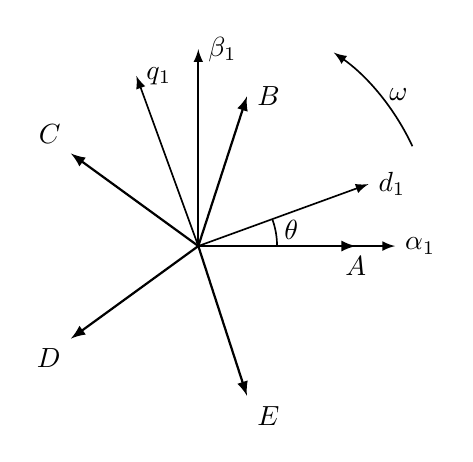
\begin{tikzpicture}[>=latex, line width=0.6pt]

\begin{scope}[shift={(0,0)}]
% Osy alpha a beta
    \draw[->] (0,0) -- (2.5,0) node[right] {$\alpha_1$};
    \draw[->] (0,0) -- (0,2.5) node[right] {$\beta_1$};
    
    % Vektory fází A-E (délka 2.0)
    \draw[->, thick] (0,0) -- (0:2) node[below] {$A$};
    \draw[->, thick] (0,0) -- (72:2) node[right] {$B$};
    \draw[->, thick] (0,0) -- (144:2) node[above left] {$C$};
    \draw[->, thick] (0,0) -- (216:2) node[below left] {$D$};
    \draw[->, thick] (0,0) -- (288:2) node[below right] {$E$};
    
    % d-q soustava (délka 2.3)
    \def\thetaang{20}
    \draw[->] (0,0) -- (\thetaang:2.3) node[right] {$d_1$};
    \draw[->] (0,0) -- (\thetaang+90:2.3) node[right] {$q_1$};
    
    % Úhel theta
    \draw (\thetaang:1.0) arc (\thetaang:0:1.0);
    \node at (10:1.2) {$\theta$};
    
    % ŠIPKA OMEGA - nyní na poloměru 3.0 (velmi daleko)
    \draw[->, bend left=30] (25:3.0) arc (25:55:3.0) node[midway, right] {$\omega$};
    
\end{scope}
\end{tikzpicture}}
				\end{figure}
				\[	f_{\alpha_1\beta_1} \equiv \frac{2}{5} \left( f_{a} + a_5 f_{b} + a_5^2 f_{c} + a_5^3 f_{d} + a_5^4 f_{e} \right)	\]
				\[	f_{d_1 q_1}= f_{\alpha_1 \beta_1} \cdot e^{-j\theta}\]
				kde $ a_5 = e^{j2\pi/5} $
		\end{column}
		\begin{column}{0.5\textwidth}
			\textbf{3. harmonická -- prostor $\alpha\beta_3$}
			\begin{figure}
				\centering
				\resizebox{!}{4cm }{
					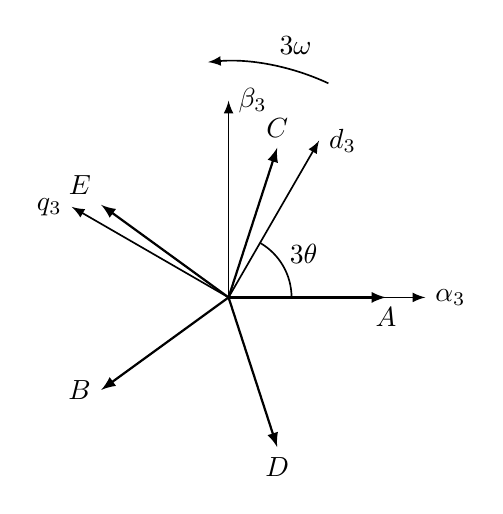
\begin{tikzpicture}[>=latex, line width=0.6pt]
\begin{scope}[shift={(7,0)}]
    % Osy alpha a beta
    \draw[->] (0,0) -- (2.5,0) node[right] {$\alpha_3$};
    \draw[->] (0,0) -- (0,2.5) node[right] {$\beta_3$};
    
    % Vektory fází A-E
    \draw[->, thick] (0,0) -- (0:2) node[below] {$A$};
    \draw[->, thick] (0,0) -- (216:2) node[left] {$B$};
    \draw[->, thick] (0,0) -- (72:2) node[above] {$C$};
    \draw[->, thick] (0,0) -- (288:2) node[below] {$D$};
    \draw[->, thick] (0,0) -- (144:2) node[above left] {$E$};
    
    % d-q soustava
    \def\threetheta{60}
    \draw[->] (0,0) -- (\threetheta:2.3) node[right] {$d_3$};
    \draw[->, shift={(0,0)}] (0,0) -- (\threetheta+90:2.3) node[left] {$q_3$};
    
    % Úhel 3*theta
    \draw (\threetheta:0.8) arc (\threetheta:0:0.8);
    \node at (30:1.1) {$3\theta$};
    
    % ŠIPKA 3*OMEGA - nyní na poloměru 3.0 (velmi daleko)
    \draw[->] (65:3.0) arc (65:95:3.0) node[midway, above right] {$3\omega$};
    
\end{scope}

\end{tikzpicture}
					}
			\end{figure}
			\[
				f_{\alpha_3\beta_3} \equiv \frac{2}{5} \left( f_{a} + a_5 f_{c} + a_5^2 f_{e} + a_5^3 f_{b} + a_5^4 f_{d} \right)
			\]
					\[	f_{d_3 q_3}= f_{\alpha_3 \beta_3} \cdot e^{-j3\theta}\]

		\end{column}
	\end{columns}
	
\end{frame}

% dq_13 matice
\begin{frame}
	\frametitle{Transformace do prostoru $dq_{1\,3}$ -- maticový zápis}
	\begin{columns}
		\begin{column}{0.5\textwidth}
			\textbf{Clarkova transformace $K_{s0}$}
			\[
				f_{\alpha \beta_{1\,3}} 
				= K_{s0} \cdot
				f_{abcde}
			\]
			\resizebox{0.9\textwidth}{!}{$K_{s0} = \frac{2}{5}
				\begin{bmatrix}
					1 & \cos\tfrac{2\pi}{5} & \cos\tfrac{4\pi}{5} & \cos\tfrac{6\pi}{5} & \cos\tfrac{8\pi}{5} \\[2pt]
					0 & \sin\tfrac{2\pi}{5} & \sin\tfrac{4\pi}{5} & \sin\tfrac{6\pi}{5} & \sin\tfrac{8\pi}{5} \\[2pt]
					1 & \cos\tfrac{6\pi}{5} & \cos\tfrac{2\pi}{5} & \cos\tfrac{8\pi}{5} & \cos\tfrac{4\pi}{5} \\[2pt]
					0 & \sin\tfrac{6\pi}{5} & \sin\tfrac{2\pi}{5} & \sin\tfrac{8\pi}{5} & \sin\tfrac{4\pi}{5} \\[2pt]
					\tfrac{1}{2} & \tfrac{1}{2} & \tfrac{1}{2} & \tfrac{1}{2} & \tfrac{1}{2}
				\end{bmatrix}$
				}
		\end{column}
		\begin{column}{0.5\textwidth}
			\textbf{Rotační matice $R_0(\theta)$}
			\[
				f_{dq_{1\,3}}
				= R_0(\theta) \cdot	f_{\alpha \beta_{1\,3}}
			\]
			\resizebox{0.9\textwidth}{!}{$
				R_0(\theta)=
				\begin{bmatrix}
					\cos\theta & \sin\theta & 0 & 0 & 0\\
					-\sin\theta & \cos\theta & 0 & 0 & 0\\
					0 & 0 & \cos 3\theta & \sin 3\theta & 0\\
					0 & 0 & -\sin 3\theta & \cos 3\theta & 0\\
					0 & 0 & 0 & 0 & 1
				\end{bmatrix}
			$}
			\vspace{0.3em}
			\textbf{Přímá transformace $K_{R0}(\theta)$}
			\[
				f_{dq_{1,3}} = \underbrace{R_0(\theta)\cdot K_{s0}}_{K_{R0}(\theta)}\cdot f_{abcde}
			\]
		\end{column}
	\end{columns}
\end{frame}

%% model v dq_13
\begin{frame}
	\frametitle{Model motoru v $dq_{1\,3}$}

	\begin{columns}[T]
		\begin{column}{0.56\textwidth}
			\textbf{Statorové napětí:}
			\begin{equation*}
				v_{dq} = R_s\,i_{dq}
					+ \omega_{fr}\,E\, \psi_{s_{dq}}+ L_s\frac{d\,i_{dq}}{dt}
			\end{equation*}
			\vspace{0.5ex}
			\textbf{Statorový tok:}
			\begin{equation*}
				\psi_{s_{dq}} =
				\underbrace{
				\begin{bmatrix}
					L_{d1}&0&0&0\\
					0&L_{q1}&0&0\\
					0&0&L_{d3}&0\\
					0&0&0&L_{q3}
				\end{bmatrix}}_{L_{s_{dq}}}
				i_{dq}
				+
				\begin{bmatrix}1\\0\\0\\0\end{bmatrix}\Psi_{PM}
			\end{equation*}
		\end{column}
		\begin{column}{0.40\textwidth}
			\textbf{Matice zpětného EMF:}
			\begin{equation*}
				E =
				\begin{bmatrix}
					0&-1&0&0\\
					1&0&0&0\\
					0&0&0&-3\\
					0&0&3&0
				\end{bmatrix}
			\end{equation*}
			\vspace{0.5ex}
			\begin{alertblock}{}
				\begin{itemize}
					\item Nezávislé na $\theta$
					\item $L_{s_{dq}}$ diagonální 
					\item $\Psi_{PM}$ pouze v ose $d_1$
				\end{itemize}
			\end{alertblock}
		\end{column}
	\end{columns}
\end{frame}

\begin{frame}
\frametitle{Odstranění křížové vazby}
\textbf{Původní model}
\begin{equation}
    \label{eq:ss idq s kriz}
     \frac{di}{dt} = \frac{1}{L_s} \left( v_{dq_{13}} - R_s i_{dq_{13}} - \omega_{fr}E \left( L_{s}i_{dq_{13}} + \gamma \Psi_{PM}\right) \right)
\end{equation}

\textbf{Substituce napětí:}
\begin{equation}
\label{eq:substituce v}
    v(t)=u(t) +  \omega(t) E \left(  i(t) + \gamma \Psi\right)
\end{equation}

\textbf{Model bez křížévé vazby}
\begin{equation}
    \label{eq:proud bez krize}
     \frac{di}{dt} = \frac{1}{L_s} \left( v - R_s i_{dq_{13}}  \right)
\end{equation}

\end{frame}

% blokac rizeni
\begin{frame}
	\frametitle{Blokové schéma řízení}
	\vfill
	\centering
\resizebox{\linewidth}{!}{%
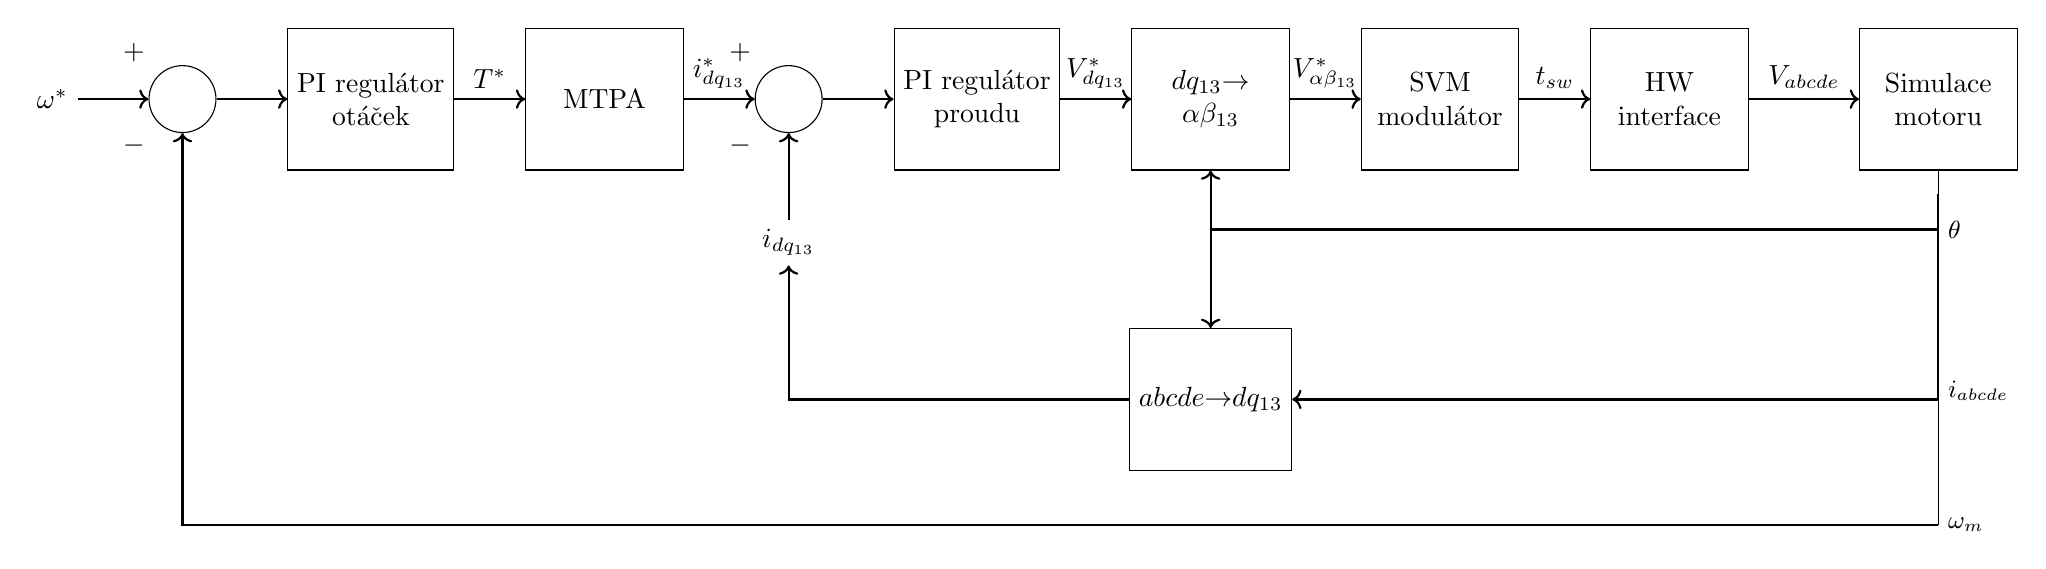
\begin{tikzpicture}[
    block/.style  = {draw, rectangle, minimum height=1.8cm, minimum width=2.0cm, align=center},
    sum/.style    = {draw, circle, minimum size=0.85cm, inner sep=0pt},
    arrow/.style  = {->, thick},
    node distance = 0.5cm and 0.9cm
]

% Dopredna cesta
\node (wref)                          {$\omega^*$};
\node[sum,   right=of wref]    (Sw)   {};
\node[block, right=of Sw]      (Rw)   {PI regulátor\\otáček};
\node[block, right=of Rw]      (MTPA) {MTPA};
\node[sum,   right=of MTPA]    (Si)   {};
\node[block, right=of Si]      (Ri)   {PI regulátor\\proudu};
\node[block, right=of Ri]      (T1)   {$dq_{13}{\to}$\\ $\alpha\beta_{13}$};
\node[block, right=of T1]      (SVM)  {SVM\\modulátor};
\node[block, right=of SVM]     (HW)   {HW\\ interface};
\node[block, right=1.4cm of HW](M)    {Simulace\\motoru};

% Zpetnovazebni transformacni blok
\node[block, below=2.0cm of T1] (T2) {$abcde{\to}dq_{13}$};

% Uzel mereneho proudu
\node[below=1.1cm of Si] (im) {$i_{dq_{13}}$};

% Znamienka sumacnich uzlu
\node[above left=2pt of Sw] {$+$};
\node[below left=2pt of Sw] {$-$};
\node[above left=2pt of Si] {$+$};
\node[below left=2pt of Si] {$-$};

% Sipky dopredne cesty
\draw[arrow] (wref) -- (Sw);
\draw[arrow] (Sw)   -- (Rw);
\draw[arrow] (Rw)   -- node[above]{$T^*$} (MTPA);
\draw[arrow] (MTPA) -- node[above]{$i^*_{dq_{13}}$} (Si);
\draw[arrow] (Si)   -- (Ri);
\draw[arrow] (Ri)   -- node[above]{$V^*_{dq_{13}}$} (T1);
\draw[arrow] (T1)   -- node[above]{$V^*_{\alpha\beta_{13}}$} (SVM);
\draw[arrow] (SVM)  -- node[above]{$t_{sw}$} (HW);
\draw[arrow] (HW)   -- node[above]{$V_{abcde}$} (M);

% Proud do sumacniho uzlu
\draw[arrow] (im) -- (Si);

% T2 -> im (vystup transformace do uzlu mereni proudu)
\draw[arrow] let \p1=(T2.west), \p2=(im.south) in
    (T2.west) -- (\x2,\y1) -- (im.south);

% Svislice z motoru
\draw let \p1=(M.south), \p2=(M.south) in
    (\x1,\y1) -- (\x1,\y1-4.50cm);

% i_abcde -> T2 (svisle dolu pak vlevo)
\node[anchor=west, font=\small]
    at ($(M.south)+(0,-2.80)$) {$i_{abcde}$};
\draw[arrow] let \p1=(M.south), \p2=(T2.east) in
    (\x1,\y1-0.30cm) -- (\x1,\y2) -- (T2.east);

% theta -> T1 a T2 (spolecna vodorovna trasa, pak vetve)
\node[anchor=west, font=\small]
    at ($(M.south)+(0,-0.75)$) {$\theta$};
\draw[arrow] let \p1=(M.south), \p2=(T1.south) in
    (\x1,\y1-0.75cm) -- (\x2,\y1-0.75cm) -- (T1.south);
\draw[arrow] let \p1=(M.south), \p2=(T2.north) in
    (\x1,\y1-0.75cm) -- (\x2,\y1-0.75cm) -- (T2.north);

% omega -> Sw (zpetna vazba vedena pod T2)
\node[anchor=west, font=\small]
    at ($(M.south)+(0,-4.50)$) {$\omega_m$};
\draw[arrow] let \p1=(M.south), \p2=(Sw.south) in
    (\x1,\y1-4.50cm) -- (\x2,\y1-4.50cm) -- (Sw.south);

\end{tikzpicture}%
}

	\vfill
	\begin{center}
		\footnotesize $T_\mathrm{S\_reg} = 50\,\text{ms}$
	\end{center}
\end{frame}

%Modulace 1
\begin{frame}
	\frametitle{SVM modulace}
	\begin{columns}
		\begin{column}{0.48\textwidth}
			\centering
			\resizebox{\textwidth}{!}{
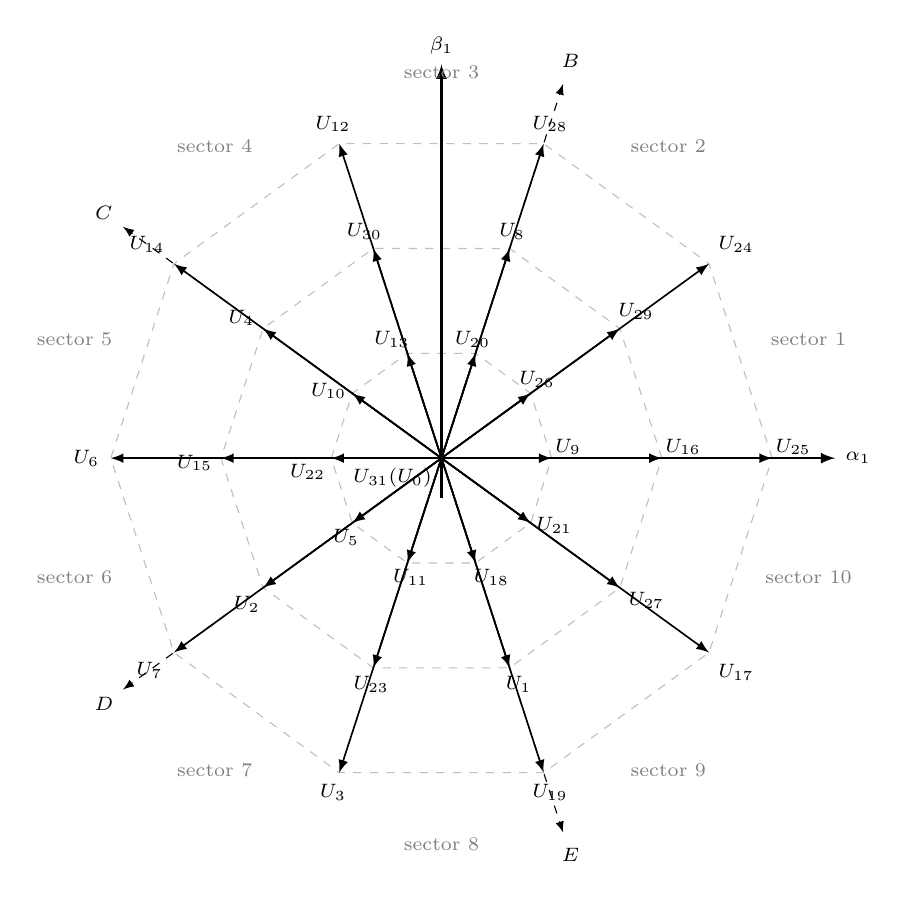
\begin{tikzpicture}[>=latex, font=\scriptsize]

    % Definice poloměrů
    \def\Rone{1.4}   
    \def\Rtwo{2.8}   
    \def\Rthree{4.2} 
    \def\Raxis{5.0}  

    % 1. Kreslení pozadí (čárkované desetiúhelníky)
    \foreach \r in {\Rone, \Rtwo, \Rthree} {
        \draw[dashed, gray!50] (0:\r) \foreach \x in {36,72,...,360} {-- (\x:\r)} -- cycle;
    }

    % 2. Hlavní osy
    \draw[->, thick] (-0.5,0) -- (\Raxis,0) node[right] {$\alpha_1$};
    \draw[->, thick] (0,-0.5) -- (0,\Raxis) node[above] {$\beta_1$};

    % Středový bod
    \node[below left] at (0,0) {$U_{31}(U_0)$};

    % 3. VEKTORY A POPISKY (Sjednocený styl pro osu alfa)

    % VNĚJŠÍ ÚROVEŇ (Level 3)
    \foreach \ang/\lab in {0/U_{25}, 36/U_{24}, 72/U_{28}, 108/U_{12}, 144/U_{14}, 180/U_6, 216/U_7, 252/U_3, 288/U_{19}, 324/U_{17}} {
        \draw[->, semithick] (0,0) -- (\ang:\Rthree);
        % Speciální podmínka pro úhel 0 (osa alfa), aby U25 bylo jako U9
        \ifnum\ang=0
            \node[anchor=south west, inner sep=1pt] at (\ang:\Rthree) {$\lab$};
        \else
            \node[anchor=\ang+180, inner sep=4pt] at (\ang:\Rthree) {$\lab$};
        \fi
    }

    % STŘEDNÍ ÚROVEŇ (Level 2)
    \foreach \ang/\lab in {0/U_{16}, 36/U_{29}, 72/U_8, 108/U_{30}, 144/U_4, 180/U_{15}, 216/U_2, 252/U_{23}, 288/U_1, 324/U_{27}} {
        \draw[->, semithick] (0,0) -- (\ang:\Rtwo);
        \ifnum\ang=0
            \node[anchor=south west, inner sep=1pt] at (\ang:\Rtwo) {$\lab$};
        \else
            \node[anchor=\ang+190, inner sep=3pt] at (\ang:\Rtwo) {$\lab$};
        \fi
    }

    % VNITŘNÍ ÚROVEŇ (Level 1)
    \foreach \ang/\lab in {0/U_9, 36/U_{26}, 72/U_{20}, 108/U_{13}, 144/U_{10}, 180/U_{22}, 216/U_5, 252/U_{11}, 288/U_{18}, 324/U_{21}} {
        \draw[->, semithick] (0,0) -- (\ang:\Rone);
        \ifnum\ang=0
            \node[anchor=south west, inner sep=1pt] at (\ang:\Rone) {$\lab$};
        \else
            \node[anchor=\ang+210, inner sep=2pt] at (\ang:\Rone) {$\lab$};
        \fi
    }

    % 4. Fázové osy a sektory
    \foreach \ang/\name in {72/B, 144/C, 216/D, 288/E} {
        \draw[->, dashed] (0,0) -- (\ang:\Raxis);
        \node at (\ang:\Raxis + 0.3) {$\name$};
    }
    
    \foreach \s/\ang in {1/18, 2/54, 3/90, 4/126, 5/162, 6/198, 7/234, 8/270, 9/306, 10/342} {
        \node[text=gray] at (\ang:\Rthree + 0.7) {sector \s};
    }


\end{tikzpicture}
}
		\end{column}
		\begin{column}{0.48\textwidth}
			\centering
			\resizebox{\textwidth}{!}{
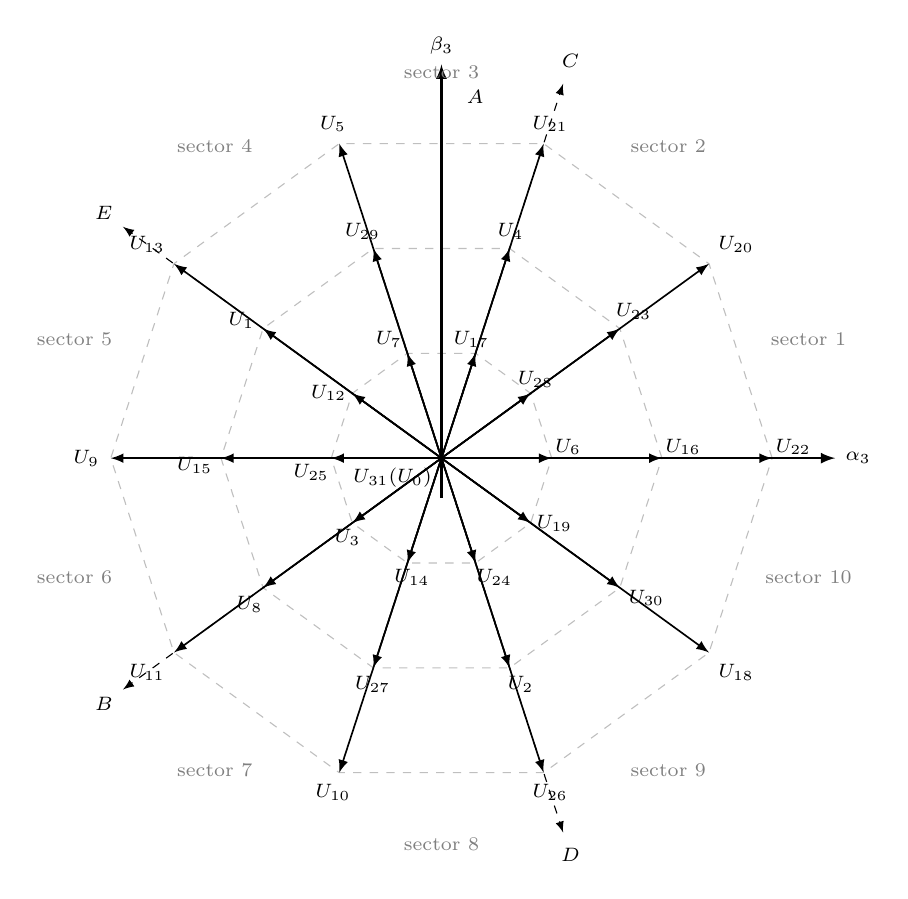
\begin{tikzpicture}[>=latex, font=\scriptsize]

    % Definice poloměrů
    \def\Rone{1.4}   
    \def\Rtwo{2.8}   
    \def\Rthree{4.2} 
    \def\Raxis{5.0}  

    % 1. Kreslení pozadí (čárkované desetiúhelníky)
    \foreach \r in {\Rone, \Rtwo, \Rthree} {
        \draw[dashed, gray!50] (0:\r) \foreach \x in {36,72,...,360} {-- (\x:\r)} -- cycle;
    }

    % 2. Hlavní osy (alfa 3 a beta 3)
    \draw[->, thick] (-0.5,0) -- (\Raxis,0) node[right] {$\alpha_3$};
    \draw[->, thick] (0,-0.5) -- (0,\Raxis) node[above] {$\beta_3$};

    % Středový bod
    \node[below left] at (0,0) {$U_{31}(U_0)$};

    % 3. VEKTORY A POPISKY PRO OBRÁZEK (b)

    % VNĚJŠÍ ÚROVEŇ (Level 3)
    \foreach \ang/\lab in {0/U_{22}, 36/U_{20}, 72/U_{21}, 108/U_{5}, 144/U_{13}, 180/U_9, 216/U_{11}, 252/U_{10}, 288/U_{26}, 324/U_{18}} {
        \draw[->, semithick] (0,0) -- (\ang:\Rthree);
        \ifnum\ang=0
            \node[anchor=south west, inner sep=1pt] at (\ang:\Rthree) {$\lab$};
        \else
            \node[anchor=\ang+180, inner sep=4pt] at (\ang:\Rthree) {$\lab$};
        \fi
    }

    % STŘEDNÍ ÚROVEŇ (Level 2)
    \foreach \ang/\lab in {0/U_{16}, 36/U_{23}, 72/U_4, 108/U_{29}, 144/U_{1}, 180/U_{15}, 216/U_{8}, 252/U_{27}, 288/U_{2}, 324/U_{30}} {
        \draw[->, semithick] (0,0) -- (\ang:\Rtwo);
        \ifnum\ang=0
            \node[anchor=south west, inner sep=1pt] at (\ang:\Rtwo) {$\lab$};
        \else
            \node[anchor=\ang+195, inner sep=3pt] at (\ang:\Rtwo) {$\lab$};
        \fi
    }

    % VNITŘNÍ ÚROVEŇ (Level 1)
    \foreach \ang/\lab in {0/U_6, 36/U_{28}, 72/U_{17}, 108/U_{7}, 144/U_{12}, 180/U_{25}, 216/U_3, 252/U_{14}, 288/U_{24}, 324/U_{19}} {
        \draw[->, semithick] (0,0) -- (\ang:\Rone);
        \ifnum\ang=0
            \node[anchor=south west, inner sep=1pt] at (\ang:\Rone) {$\lab$};
        \else
            \node[anchor=\ang+215, inner sep=2pt] at (\ang:\Rone) {$\lab$};
        \fi
    }

    % 4. Fázové osy pro (b) - A, C, E, B, D
    \node[anchor=north west] at (0.2, \Raxis-0.2) {$A$}; % Label u osy alfa
    \foreach \ang/\name in {72/C, 144/E, 216/B, 288/D} {
        \draw[->, dashed] (0,0) -- (\ang:\Raxis);
        \node at (\ang:\Raxis + 0.3) {$\name$};
    }
    
    % 5. Sektory
    \foreach \s/\ang in {1/18, 2/54, 3/90, 4/126, 5/162, 6/198, 7/234, 8/270, 9/306, 10/342} {
        \node[text=gray] at (\ang:\Rthree + 0.7) {sector \s};
    }



\end{tikzpicture}
}
		\end{column}
	\end{columns}
	\vspace{0.5em}
	\begin{columns}
		\begin{column}{0.55\textwidth}
			\begin{itemize}
				\item 32 výstupních vektorů (10 sektorů)
			\end{itemize}
		\end{column}
		
	\end{columns}
\end{frame}

%Modulace 2
\begin{frame}
	\frametitle{SVM modulace}
	\begin{columns}
		\begin{column}{0.5\textwidth}
		\begin{itemize}
			\item výběr 4 nenulovách na základě $U_{\alpha\beta _1}^*$ 
			\item Nejdelší v $\alpha\beta_1$ odpovídá nejkratšímu v $\alpha\beta_3$
		\end{itemize}


		\begin{equation*}
			\label{eq:maticove svm}
			U_{\alpha \beta_{13}}^*=A \cdot 
			\begin{bmatrix}
				t_1\\t_2\\t_3\\t_4   
			\end{bmatrix}
		\end{equation*}
		\begin{equation*}
			\label{eq:svm casy final}
			t_{vec}
			= A_n^{-1}\cdot  U_{\alpha \beta_{1\,3}}^*
		\end{equation*}

		\end{column}
		\begin{column}{0.3\textwidth}
			\vspace{-0.5em}
			\begin{figure}
				% První obrázek
					\centering
					\resizebox{!}{0.5\height}{
						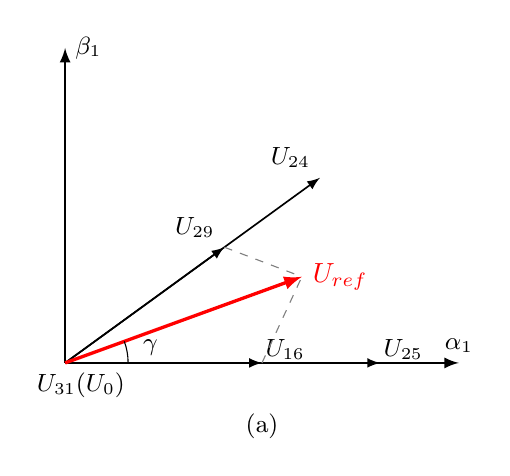
\begin{tikzpicture}[>=latex, font=\small]

    % Osy
    \draw[->, thick] (0,0) -- (5,0) node[above] {$\alpha_1$};
    \draw[->, thick] (0,0) -- (0,4) node[right] {$\beta_1$};
    \node[below] at (0.2,0) {$U_{31}(U_0)$};

    % Definice délek
    \def\Lone{2.5} 
    \def\Ltwo{4.0} 
    \def\Lref{3.2} 
    \def\angRef{20}

    % Vektory na ose alfa (U16, U25) - umístění nad šipkou
    \draw[->, semithick] (0,0) -- (\Lone,0) node[anchor=south west, inner sep=1pt] {$U_{16}$};
    \draw[->, semithick] (0,0) -- (\Ltwo,0) node[anchor=south west, inner sep=1pt] {$U_{25}$};

    % Vektory pod úhlem (U29, U24)
    \draw[->, semithick] (0,0) -- (36:\Lone) node[anchor=south east] {$U_{29}$};
    \draw[->, semithick] (0,0) -- (36:\Ltwo) node[anchor=south east] {$U_{24}$};

    % ČERVENÝ REFERENČNÍ VEKTOR Uref
    \draw[->, very thick, red] (0,0) -- (\angRef:\Lref) node[right, font=\bfseries] {$U_{ref}$};

    % Úhel gama
    \draw (0.8,0) arc (0:\angRef:0.8);
    \node at (10:1.1) {$\gamma$};

    % Konstrukční čáry
    \draw[dashed, gray] (36:\Lone) -- (\angRef:\Lref);
    \draw[dashed, gray] (\Lone,0) -- (\angRef:\Lref);

    \node at (2.5, -0.8) {(a)};

\end{tikzpicture}
					}
				\end{figure}
				\begin{figure}
				% Druhý obrázek
					\centering
					\resizebox{!}{0.5\height}{
						\begin{tikzpicture}[>=latex, font=\small]

    % Osy
    \draw[->, thick] (-2.5,0) -- (4.5,0) node[below] {$\alpha_3$};
    \draw[->, thick] (0,-2.5) -- (0,4) node[right] {$\beta_3$};
    \node[anchor=south west, xshift=2pt] at (0,0) {$U_{31}(U_0)$};

    % Vektory na ose (U16 vpravo, U25 vlevo)
    \draw[->, semithick] (0,0) -- (2.8,0) node[anchor=south west, inner sep=1pt] {$U_{16}$};
    \draw[->, semithick] (0,0) -- (-1.8,0) node[anchor=north east] {$U_{25}$};

    % Šikmé vektory (U29 a U24)
    \draw[->, semithick] (0,0) -- (108:3.0) node[anchor=south east] {$U_{29}$};
    \draw[->, semithick] (0,0) -- (288:2.2) node[anchor=north west] {$U_{24}$};

    % ČERVENÝ REFERENČNÍ VEKTOR Uref3
    \def\angRefThree{130}
    \def\LrefThree{1.5}
    \draw[->, very thick, red] (0,0) -- (\angRefThree:\LrefThree) node[anchor=south east, font=\bfseries] {$U_{ref3}$};



\end{tikzpicture}
					}
				\end{figure}
		\end{column}
	\end{columns}


\end{frame}

%Modulace implmentace
\begin{frame}
	\frametitle{Implementace SVPWM}
	\begin{figure}
		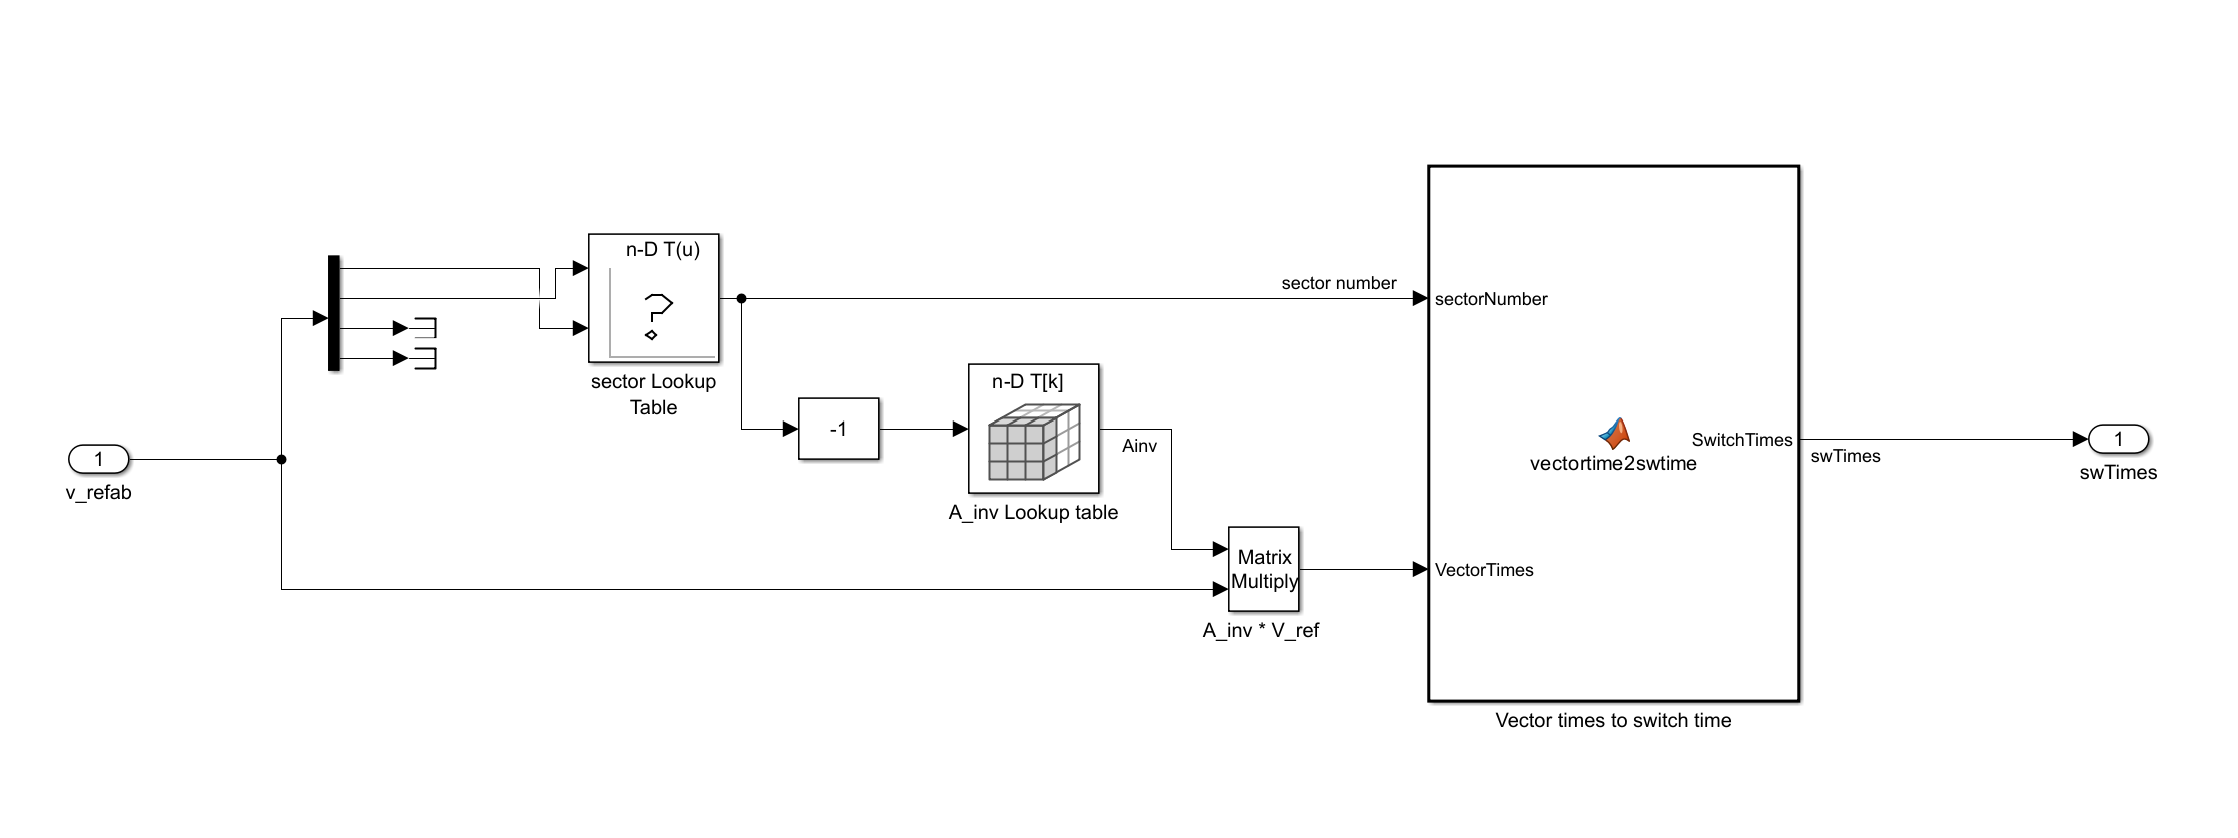
\includegraphics[width=\linewidth]{obrazky/svm_simulink.png}
	\end{figure}

	$	t_{vec}	= A_n^{-1}\cdot  U_{\alpha \beta_{1\,3}}^*	$
\end{frame}

%% MTPA 1
\begin{frame}
	\frametitle{Generování proudové reference MTPA }
	\textbf{Generovaný moment:}
		\begin{equation}
			\label{eq:moment 3rd}
			T_e = \frac{5}{2} p \cdot \left[
			\Big(\Psi _{\mathrm{PM}}+i_{\mathrm{d1}}\,\big(L_{\mathrm{d1}}-L_{\mathrm{q1}}\big)\Big)\,i_{\mathrm{q1}}+
			\Big( k\cdot \Psi_{PM}+ i_{\mathrm{d3}} \big(L_{\mathrm{d3}}-\,L_{\mathrm{q3}}\big)\Big)3\,i_{\mathrm{q3}}\right]
		\end{equation}

	\textbf{Minimalizace oporových ztrát $P=I^2 R$:}	
	\begin{equation}
		\label{eq:optimalni proud}
		J_{min} = i_{d1}^2 + i_{q1}^2 + i_{d3}^2 + i_{q3}^2
	\end{equation}

	\textbf{Omezení proudu:}
	\begin{equation}
		\label{eq:Idc max}
		\sqrt{i_{d1}^2 + i_{q1}^2 + i_{d3}^2 + i_{q3}^2} \leq I_{DC\text{max}}
	\end{equation}

	\begin{equation}
		\label{eq:isw max}
		i_{n,\text{max}} \geq \hat{I}_1 + \hat{I}_3 = \sqrt{i_{d1}^2 + i_{q1}^2} + \sqrt{i_{d3}^2 + i_{q3}^2}
	\end{equation}
\end{frame}

% MTPA 2
\begin{frame}
	\frametitle{Generování proudové reference MTPA -- pokračování}

	\begin{columns}
		\begin{column}{0.35\textwidth}
			\begin{alertblock}{Poronání \\ maximláních  mometů}
			
					\begin{tabular}{lccc}
						Pouze $i_{q1}$                 &  9{,}8 Nm    \\
						$i_{dq_1}$  & 14{,}76 Nm \\
						$i_{dq_{1\,3}}$  & 17{,}88 Nm\\

						
					\end{tabular}
				
			\end{alertblock}
			\begin{itemize}
				\item Problém řešnen matlab funkci \texttt{fmincon} 
				\item Implmenatce jako Lookup tabulka 
			\end{itemize}
		\end{column}
		\begin{column}{0.7\textwidth}
			\begin{figure}
				\centering
				\includegraphics[width=\textwidth]{obrazky/mtpa3.png}
				\caption{Optimální proudy s injekcí 3.~harmonické}
			\end{figure}
			
		\end{column}
	\end{columns}
\end{frame}









%%%%%%%%%%%%%
% Snímek 8a: Výsledky simulace -- průběh otáček a zátěže
\begin{frame}
	\frametitle{Výsledky simulace -- regulace otáček}
	\textbf{Podmínky:} skokové změny otáček každých 5\,s, přídavná zátěž 0--5\,Nm (perioda 2{,}5\,s), $T_s=50\,\mu\text{s}$
	\vspace{0.5ex}
	\begin{figure}
		\centering
		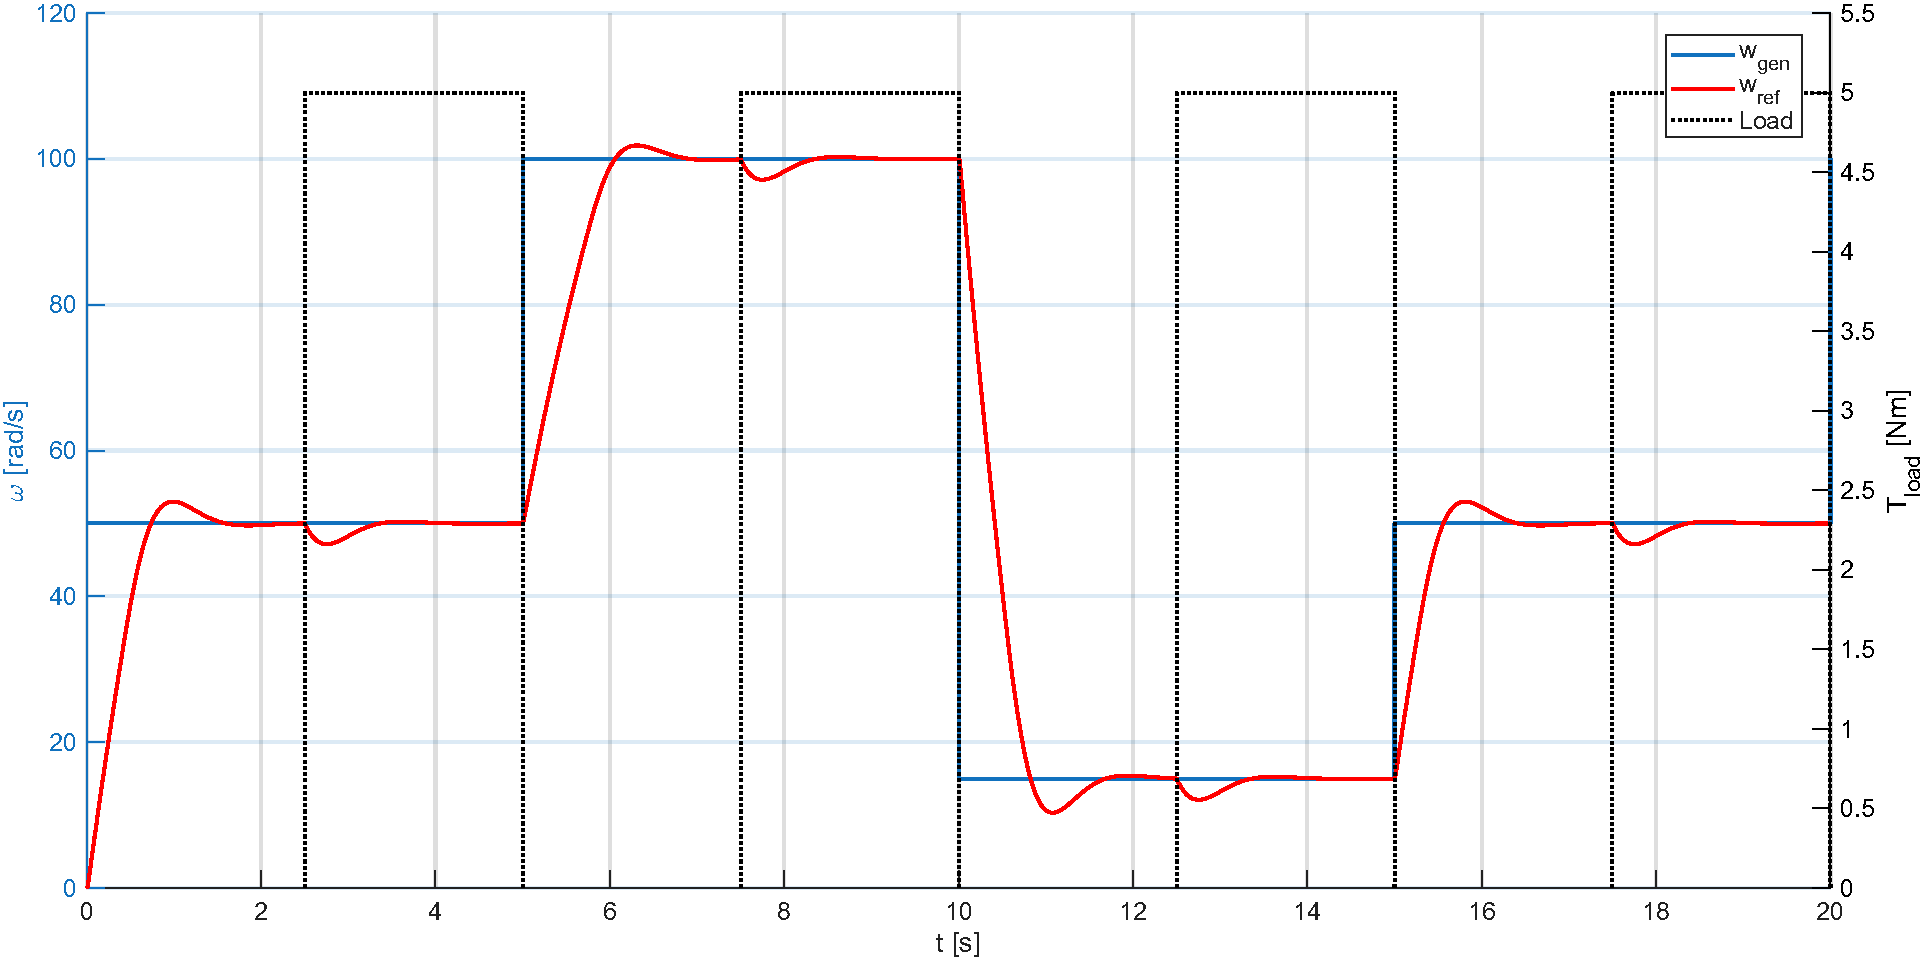
\includegraphics[width=0.95\textwidth]{obrazky/speedReg2}
		\caption{Průběh rychlosti a zátěžného momentu}
	\end{figure}
	\begin{itemize}
		\item Regulátor rychle sleduje skok žádané hodnoty
		\item Kompenzace poruchového momentu (přídavná zátěž) díky I-složce regulátoru otáček
	\end{itemize}
\end{frame}


%%%%%%%%%%%%%
% Snímek 8b: Výsledky simulace -- průběh momentu
\begin{frame}
	\frametitle{Výsledky simulace -- průběh momentu}
	\begin{figure}
		\centering
		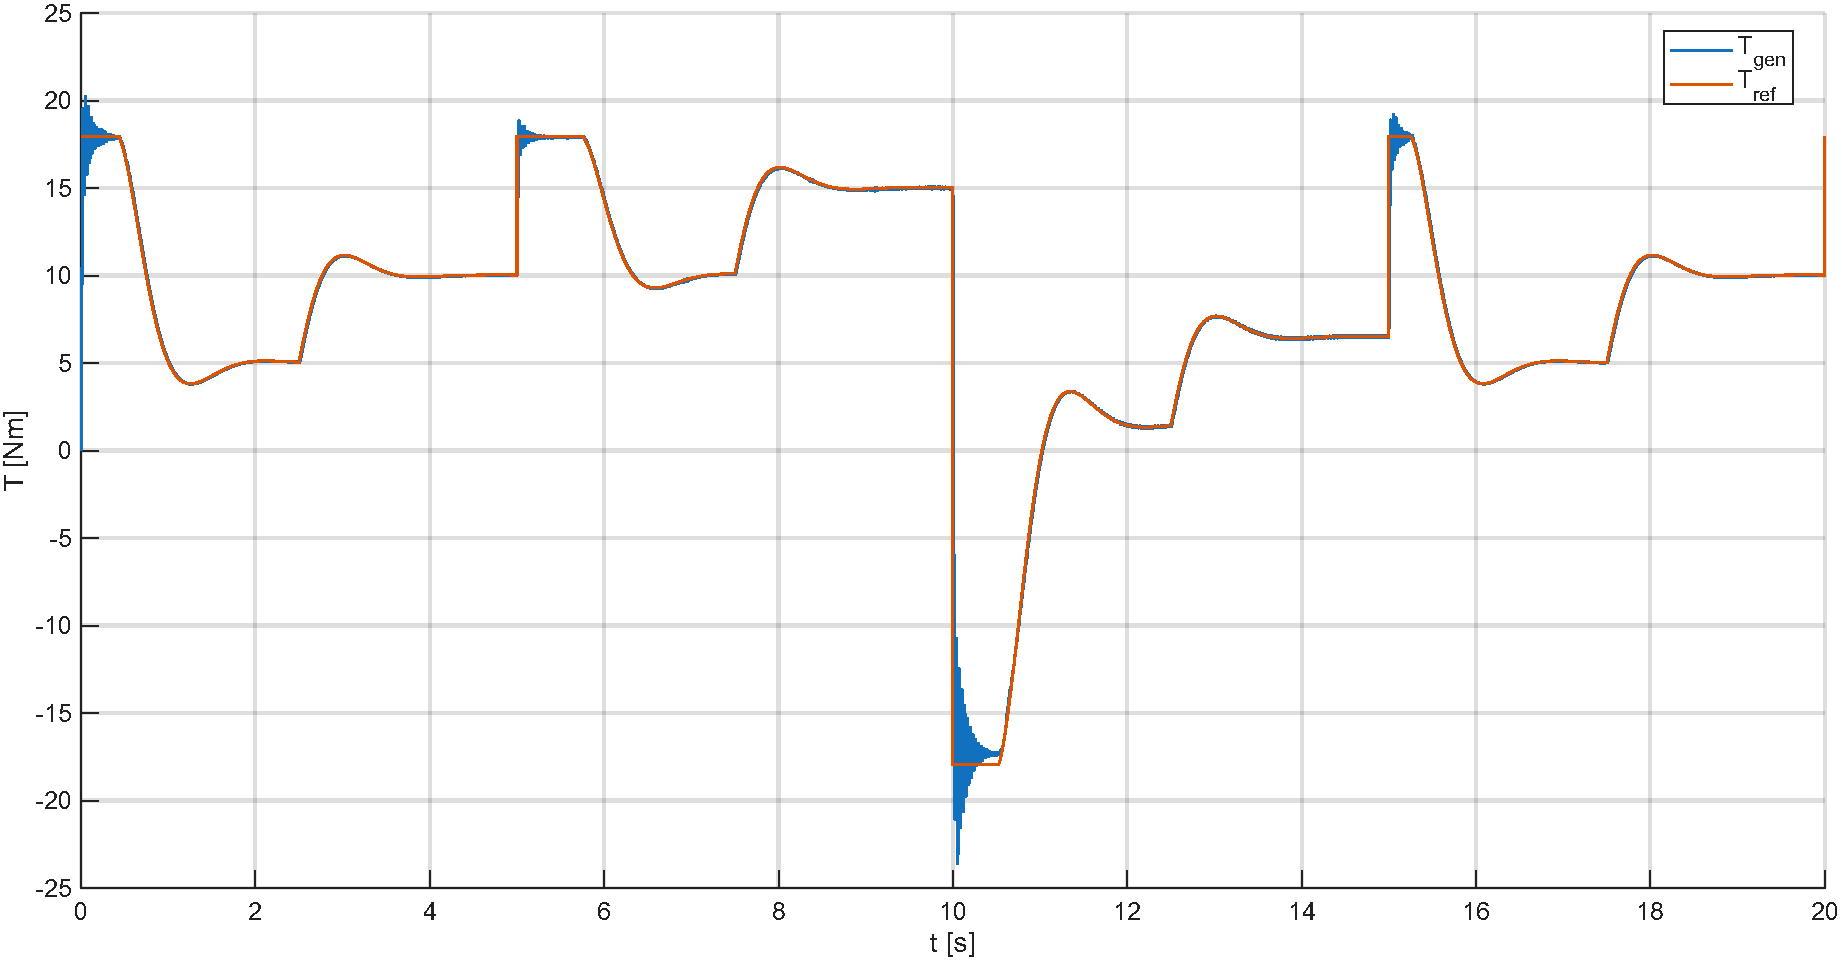
\includegraphics[width=0.95\textwidth]{obrazky/speedReg1}
		\caption{Průběh žádaného a skutečného momentu}
	\end{figure}
	\begin{columns}[T]
		\begin{column}{0.5\textwidth}
			\begin{itemize}
				\item Skutečný moment sleduje žádanou hodnotu bez přeregulování
				\item Filtr žádaného momentu ($\tau=50\,\text{ms}$) eliminuje proudové překmity
			\end{itemize}
		\end{column}
		\begin{column}{0.5\textwidth}
			\begin{block}{Vlastní model motoru}
				Simscape nezahrnuje 3.~harmonickou $\Rightarrow$ vlastní analytický model v $dq_{1\,3}$
			\end{block}
		\end{column}
	\end{columns}
\end{frame}


%%%%%%%%%%%%%
% Snímek 9: FPGA implementace -- ZedBoard
\begin{frame}
	\frametitle{Implementace na FPGA -- ZedBoard}
	\begin{columns}[T]
		\begin{column}{0.56\textwidth}
			\begin{itemize}
				\item \textbf{ZedBoard}: Xilinx Zynq-7020 (ARM Cortex-A9 + FPGA Artix-7)
				\item IP cores generovány nástrojem \textbf{Matlab HDL Coder}
				\item Uprava kódu 
					\begin{itemize}
						\item definovány odpovidající dat tipy
						\item pouze funkce podoporujicí HDL Coder
						\item minimalizce počtu sin cos výpočtů
						\end{itemize}
				\item Funkčnost ověřena pomocí \textbf{HIL simulace} (Ethernet)
				\item Výstup na fyzické piny 
				\item \textbf{Dead-time} při přepínání (zamezení zkratu větve)
			\end{itemize}
		\end{column}
		\begin{column}{0.44\textwidth}
			\begin{figure}
				\centering
				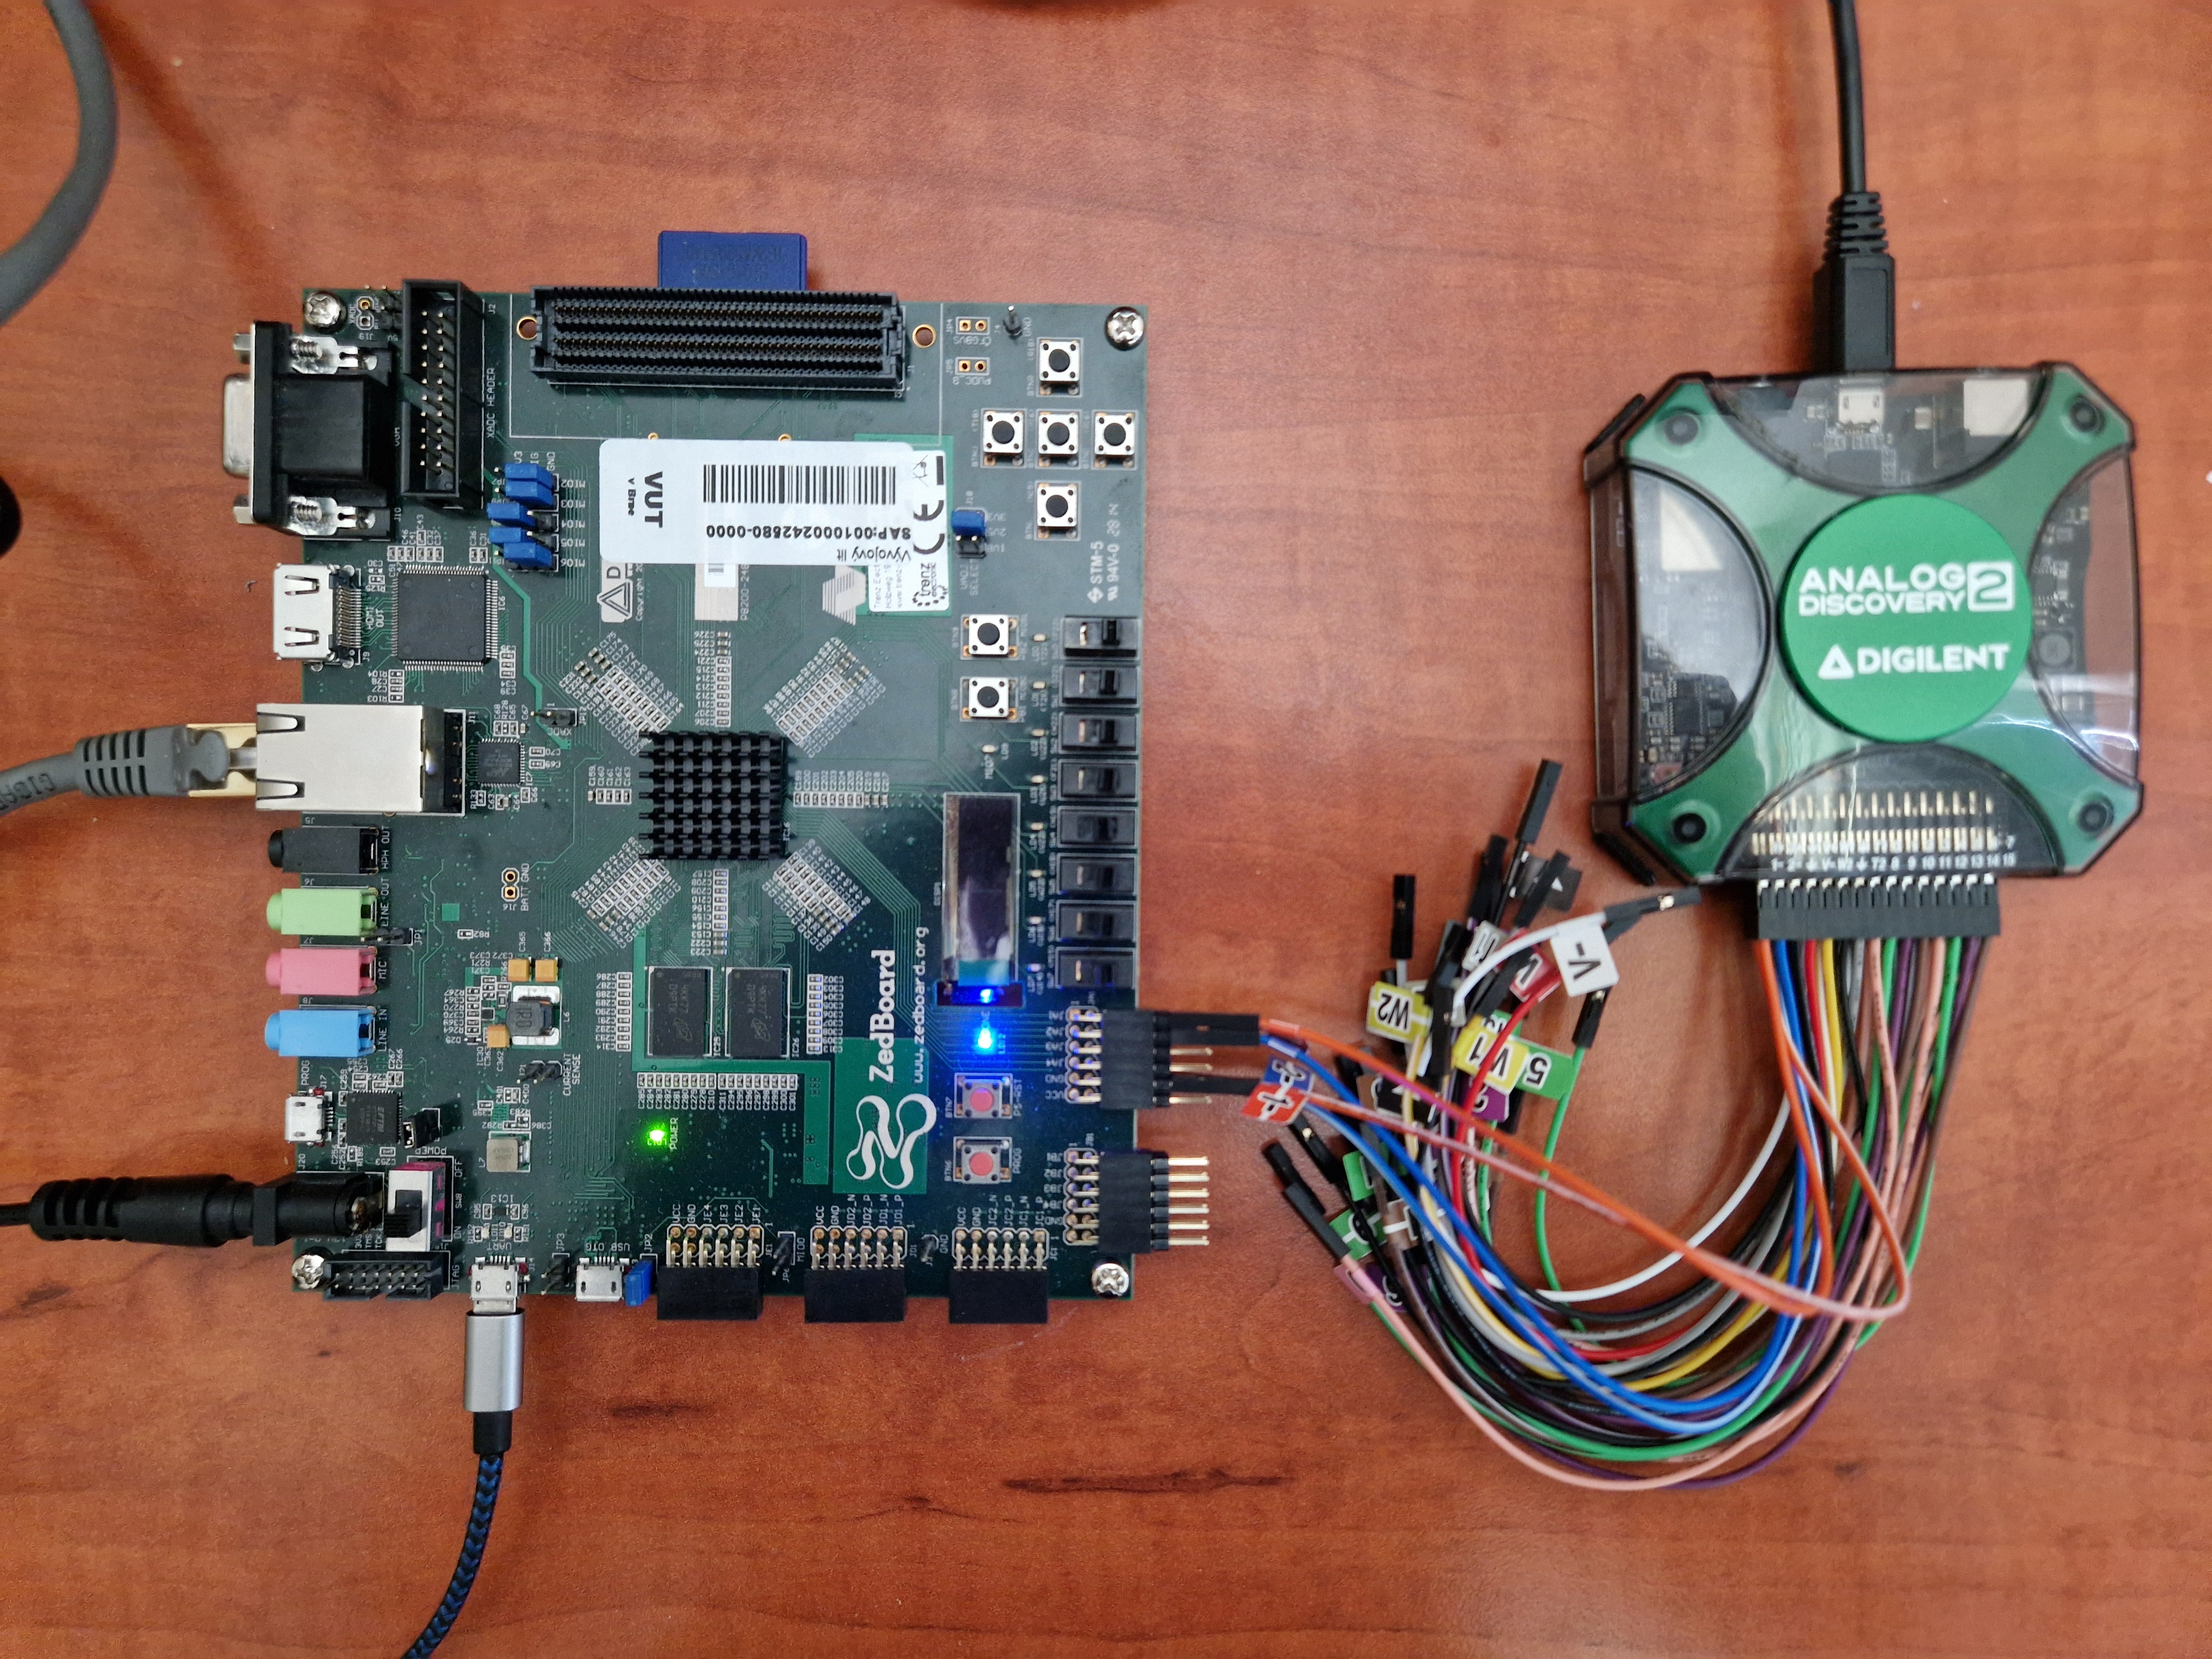
\includegraphics[width=0.9\columnwidth]{obrazky/zedBoard.jpg}
			\end{figure}
		\end{column}
	\end{columns}
\end{frame}




%%%%%%%%%%%%%
% Snímek 11: Závěr
\begin{frame}
	\frametitle{Závěr}
	\begin{itemize}
		\item Odvozena a implementována {rozšířená transformace $dq_{1\,3}$} pětifázového PMSM
		\item Navržen a ověřen {SVPWM modulátor} 
		\item Implementován {kaskádní regulátor} s kompenzací křížové vazby
		\item {MTPA s injekcí 3.~harmonické}
		\item Vytvořena simulink knihovna s jednotlivými bloky ve spojité i diskrétní formě
		\item Celé řízení {nasazeno na FPGA ZedBoard} a ověřeno HIL simulací
		
	\end{itemize}
	\vspace{1ex}
	\begin{block}{Možná rozšíření}
		\begin{itemize}
			\item Oslabování magnetického pole (MTPV) pro provoz nad $\omega_{base}$
			\item Reakce na výpadek jedné z fází
		\end{itemize}
	\end{block}
\end{frame}


%%%%%%%%%%%%%
% Poděkování
\begin{frame}[c]
	\frametitle{\mbox{ }}
	\begin{center}
		{\Huge Děkuji za pozornost!}
	\end{center}
\end{frame}


%%%%%%%%%%%%%
% Otázky oponenta
\begin{frame}[plain,noframenumbering]
	\frametitle{Otázka oponenta 1}
	\emph{Pro úpravu požadované hodnoty používáte jednoduchý setrvačný článek, zkoušel jste také úpravu požadované hodnoty pomocí rampy? Jaké jsou výhody/nevýhody obou přístupů?}\\[2ex]
	%
	\begin{columns}[T]
		\begin{column}{0.48\textwidth}
			\textbf{Setrvačný článek}
			\begin{itemize}
				\item Plynulý přechod 
				\item Snažší implementace
				\item Výstup asymptoticky konverguje k žádané hodnotě, nikdy jí přesně nedosáhne
				\item Při velkých skocích může být přechodový děj nepříjemně dlouhý
			\end{itemize}
		\end{column}
		\begin{column}{0.48\textwidth}
			\textbf{Rampa}
			\begin{itemize}
				\item Lineární průběh 
				\item Žádaná hodnota je dosažena přesně po konečném čase
				\item Parametr sklonu přímo odpovídá maximální rychlosti změny
				\item Na konci rampy vzniká skok derivace 
				\item Zanáší nelinearizu do systému
			\end{itemize}
		\end{column}
	\end{columns}

\end{frame}


\begin{frame}[plain,noframenumbering]
	\frametitle{Otázka oponenta 2}
	\emph{Z Obr. 2.2 není zcela jasné, zda byly jednotlivé průběhy měřeny nezávisle na sobě, nebo všechny naráz. Upřesněte komisi proces, kterým byly získány naměřené průběhy přechodových charakteristik.
}\\[2ex]
	%
\end{frame}

\begin{frame}
	
	\begin{figure}
		\centering
		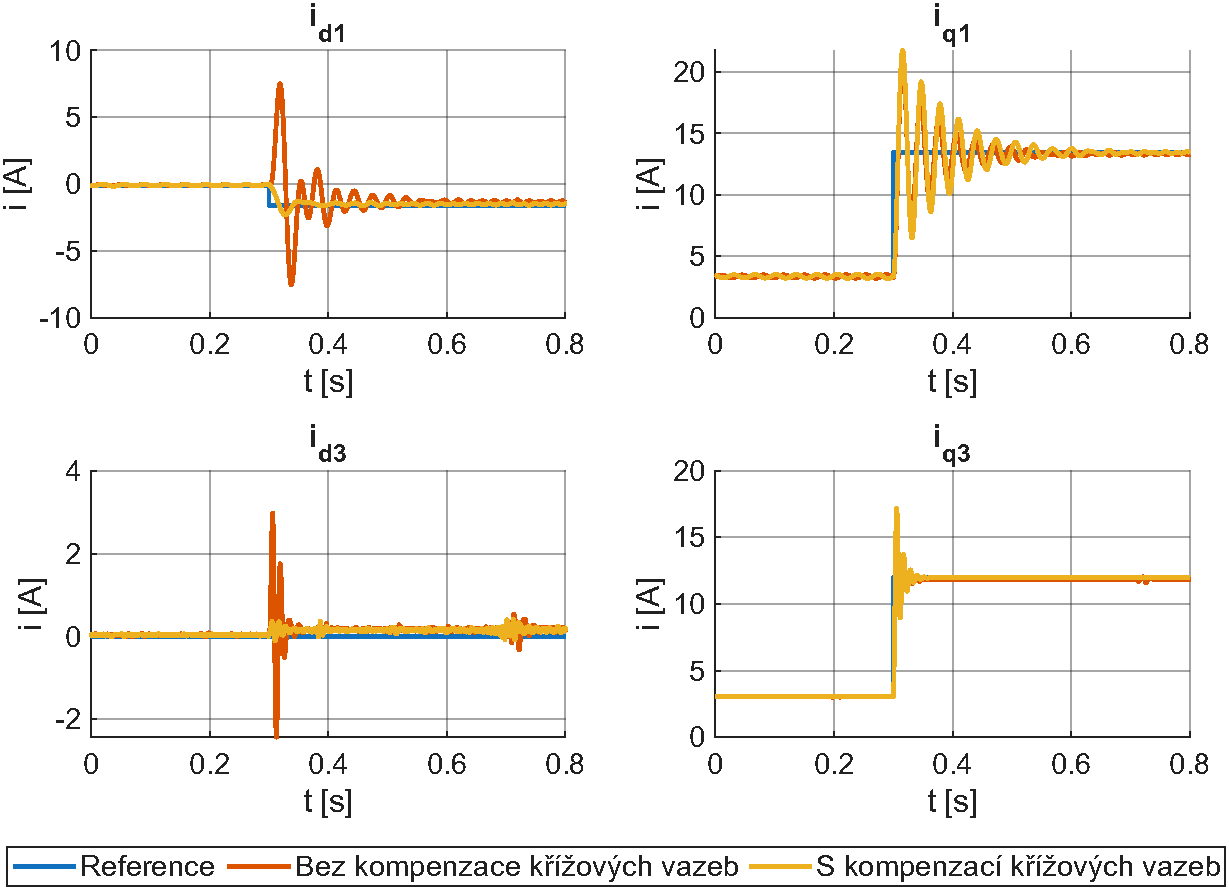
\includegraphics[width=0.9\textwidth]{obrazky/cross_compens_prez.pdf}
	\end{figure}
\end{frame}

\begin{frame}[plain,noframenumbering]
	\frametitle{Otázka oponenta 3}
	\emph{Co způsobuje záporné časy sepnutí u výstupu z funkce vectortime2swtime?}\\[2ex]
	%
	\begin{columns}
		\begin{column}{0.5\textwidth}
			
			\begin{figure}
				\centering
				% První obrázek
				
					\centering
					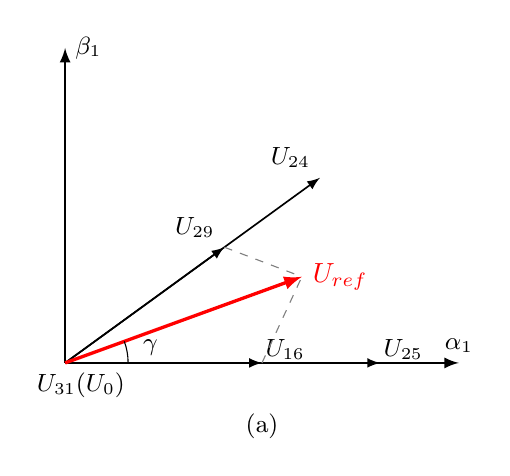
\begin{tikzpicture}[>=latex, font=\small]

    % Osy
    \draw[->, thick] (0,0) -- (5,0) node[above] {$\alpha_1$};
    \draw[->, thick] (0,0) -- (0,4) node[right] {$\beta_1$};
    \node[below] at (0.2,0) {$U_{31}(U_0)$};

    % Definice délek
    \def\Lone{2.5} 
    \def\Ltwo{4.0} 
    \def\Lref{3.2} 
    \def\angRef{20}

    % Vektory na ose alfa (U16, U25) - umístění nad šipkou
    \draw[->, semithick] (0,0) -- (\Lone,0) node[anchor=south west, inner sep=1pt] {$U_{16}$};
    \draw[->, semithick] (0,0) -- (\Ltwo,0) node[anchor=south west, inner sep=1pt] {$U_{25}$};

    % Vektory pod úhlem (U29, U24)
    \draw[->, semithick] (0,0) -- (36:\Lone) node[anchor=south east] {$U_{29}$};
    \draw[->, semithick] (0,0) -- (36:\Ltwo) node[anchor=south east] {$U_{24}$};

    % ČERVENÝ REFERENČNÍ VEKTOR Uref
    \draw[->, very thick, red] (0,0) -- (\angRef:\Lref) node[right, font=\bfseries] {$U_{ref}$};

    % Úhel gama
    \draw (0.8,0) arc (0:\angRef:0.8);
    \node at (10:1.1) {$\gamma$};

    % Konstrukční čáry
    \draw[dashed, gray] (36:\Lone) -- (\angRef:\Lref);
    \draw[dashed, gray] (\Lone,0) -- (\angRef:\Lref);

    \node at (2.5, -0.8) {(a)};

\end{tikzpicture}
					\caption{Prostor $\alpha \, \beta \,1$ }
					\label{fig:svm detail vlevo}
				\end{figure}
				
			\end{column}
			\begin{column}{0.5\textwidth}
				\begin{figure}
					\centering
					\resizebox{!}{0.75\height}{
					\begin{tikzpicture}[>=latex, font=\small]

    % Osy
    \draw[->, thick] (-2.5,0) -- (4.5,0) node[below] {$\alpha_3$};
    \draw[->, thick] (0,-2.5) -- (0,4) node[right] {$\beta_3$};
    \node[anchor=south west, xshift=2pt] at (0,0) {$U_{31}(U_0)$};

    % Vektory na ose (U16 vpravo, U25 vlevo)
    \draw[->, semithick] (0,0) -- (2.8,0) node[anchor=south west, inner sep=1pt] {$U_{16}$};
    \draw[->, semithick] (0,0) -- (-1.8,0) node[anchor=north east] {$U_{25}$};

    % Šikmé vektory (U29 a U24)
    \draw[->, semithick] (0,0) -- (108:3.0) node[anchor=south east] {$U_{29}$};
    \draw[->, semithick] (0,0) -- (288:2.2) node[anchor=north west] {$U_{24}$};

    % ČERVENÝ REFERENČNÍ VEKTOR Uref3
    \def\angRefThree{130}
    \def\LrefThree{1.5}
    \draw[->, very thick, red] (0,0) -- (\angRefThree:\LrefThree) node[anchor=south east, font=\bfseries] {$U_{ref3}$};



\end{tikzpicture}
					}
					\caption{Prostor $\alpha \, \beta \,3$}
					\label{fig:svm detail vpravo}
				\end{figure}
				
				
			
			\end{column}
		\end{columns}
\end{frame}

\end{document}
